%%%%%%%%%%%%%%%%%%%%%%%%%%%%%%%%%%%%%%%%%
% Beamer Presentation
% LaTeX Template
% Version 1.0 (10/11/12)
%
% This template has been downloaded from:
% http://www.LaTeXTemplates.com
%
% License:
% CC BY-NC-SA 3.0 (http://creativecommons.org/licenses/by-nc-sa/3.0/)
%
%%%%%%%%%%%%%%%%%%%%%%%%%%%%%%%%%%%%%%%%%

%----------------------------------------------------------------------------------------
%	PACKAGES AND THEMES
%----------------------------------------------------------------------------------------

\documentclass{beamer}

\mode<presentation> {

% The Beamer class comes with a number of default slide themes
% which change the colors and layouts of slides. Below this is a list
% of all the themes, uncomment each in turn to see what they look like.

%\usetheme{default}
%\usetheme{AnnArbor}
%\usetheme{Antibes}
%\usetheme{Bergen}
%\usetheme{Berkeley}
%\usetheme{Berlin}
%\usetheme{Boadilla}
%\usetheme{CambridgeUS}
%\usetheme{Copenhagen}
%\usetheme{Darmstadt}
%\usetheme{Dresden}
%\usetheme{Frankfurt}
%\usetheme{Goettingen}
%\usetheme{Hannover}
%\usetheme{Ilmenau}
%\usetheme{JuanLesPins}
%\usetheme{Luebeck}
\usetheme{Madrid}
%\usetheme{Malmoe}
%\usetheme{Marburg}
%\usetheme{Montpellier}
%\usetheme{PaloAlto}
%\usetheme{Pittsburgh}
%\usetheme{Rochester}
%\usetheme{Singapore}
%\usetheme{Szeged}
%\usetheme{Warsaw}

% As well as themes, the Beamer class has a number of color themes
% for any slide theme. Uncomment each of these in turn to see how it
% changes the colors of your current slide theme.

%\usecolortheme{albatross}
%\usecolortheme{beaver}
%\usecolortheme{beetle}
%\usecolortheme{crane}
%\usecolortheme{dolphin}
%\usecolortheme{dove}
%\usecolortheme{fly}
%\usecolortheme{lily}
%\usecolortheme{orchid}
%\usecolortheme{rose}
%\usecolortheme{seagull}
%\usecolortheme{seahorse}
%\usecolortheme{whale}
%\usecolortheme{wolverine}

%\setbeamertemplate{footline} % To remove the footer line in all slides uncomment this line
%\setbeamertemplate{footline}[page number] % To replace the footer line in all slides with a simple slide count uncomment this line

%\setbeamertemplate{navigation symbols}{} % To remove the navigation symbols from the bottom of all slides uncomment this line
}

\usepackage{graphicx} % Allows including images
\usepackage{booktabs} % Allows the use of \toprule, \midrule and \bottomrule in tables
\usepackage{multirow}
\usepackage{adjustbox}
\usepackage{array}
\usepackage{tikz}
\usepackage{soul}
\usetikzlibrary{shapes.geometric, arrows, positioning, fit}
\usepackage[latin1]{inputenc}
\newcommand{\xmark}{\textcolor{red}{\text{\sffamily X}}}
\newcommand{\cmark}{\textcolor{green}{\checkmark}}
\newcommand{\tr}{\text{tr}}
\newcommand{\E}{\textbf{E}}
\newcommand{\diag}{\text{diag}}
\newcommand{\argmax}{\text{argmax}}
\newcommand{\argmin}{\text{argmin}}
\newcommand{\Cov}{\text{Cov}}
\newcommand{\Var}{\text{Var}}
\newcommand{\Vol}{\text{Vol}}
\newcommand{\bx}{\boldsymbol{x}}
\newcommand{\by}{\boldsymbol{y}}
\newcommand{\bX}{\boldsymbol{X}}
\newcommand{\bY}{\boldsymbol{Y}}
\sethlcolor{gray}
\makeatletter
\newcommand\SoulColor{%
  \let\set@color\beamerorig@set@color
  \let\reset@color\beamerorig@reset@color}
\makeatother
\definecolor{color1}{RGB}{128,0,0}
\definecolor{color2}{RGB}{0,128,0}
\definecolor{color3}{RGB}{0,0,128}
\definecolor{color4}{RGB}{70,13,128}

%tikz stufff


%----------------------------------------------------------------------------------------
%	TITLE PAGE
%----------------------------------------------------------------------------------------


\title[Informal]{Causal Inference and Invariance}

\author{Charles Zheng and Qingyuan Zhao}
\institute[Stanford]
{Stanford University}
\date{\today}

\begin{document}

\begin{frame}
\titlepage
(Part 1/2)
\end{frame}












\section{Introduction}

\begin{frame}
\frametitle{Understanding = cause and effect}
\begin{tabular}{cc}
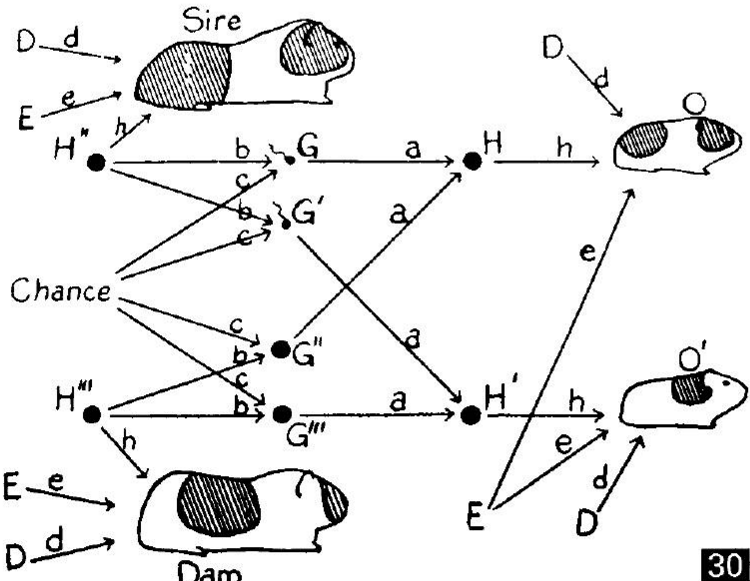
\includegraphics[scale=0.13]{../images/pearl30.png}& \\
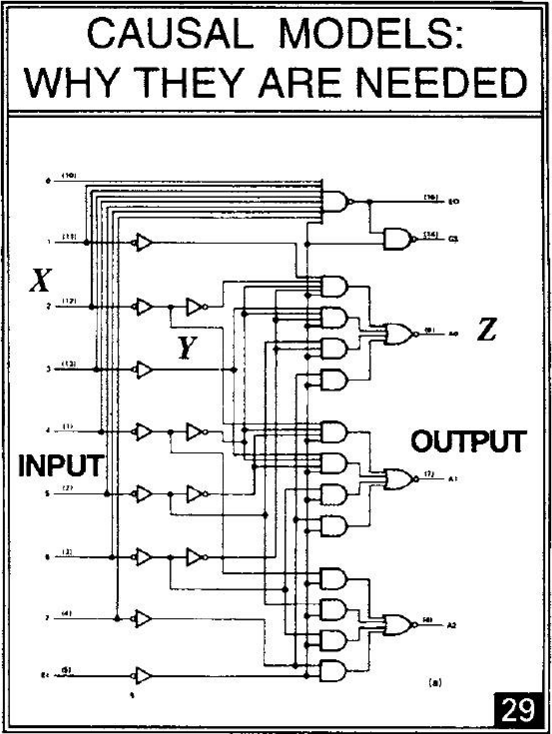
\includegraphics[scale=0.17]{../images/pearl29.png} &
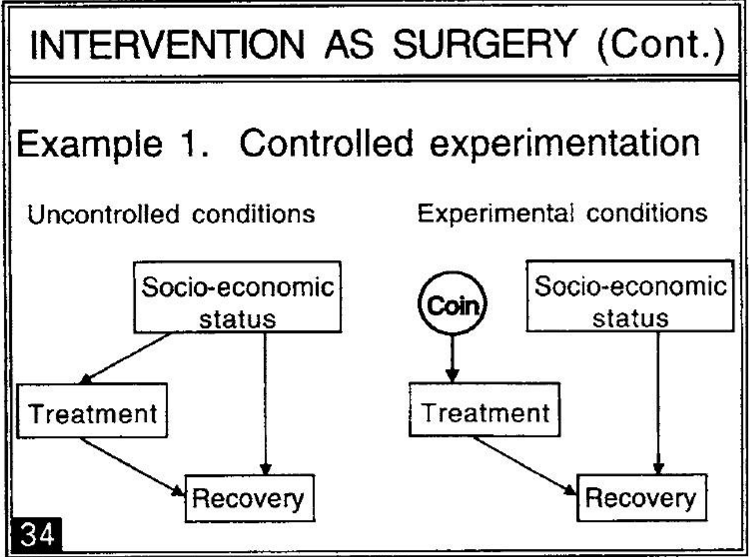
\includegraphics[scale=0.25]{../images/pearl34.png}
\end{tabular}
\end{frame}

\begin{frame}
\frametitle{A hot application: systems biology}
\begin{center}
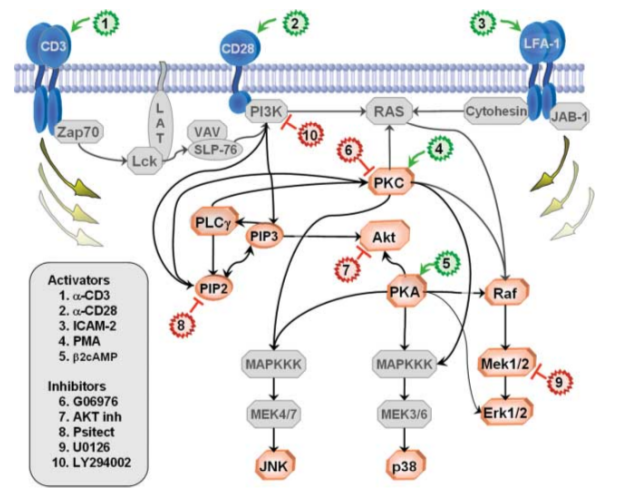
\includegraphics[scale=0.3]{../images/cyto_graph.png}
\end{center}
\begin{itemize}
\item Causal relationships = \emph{chemical interactions}.
\item Experimenters \emph{intervene} by injecting \emph{activators} and \emph{inhibitors}.
\end{itemize}
\end{frame}

\begin{frame}
\frametitle{Protein signalling data}
\begin{center}
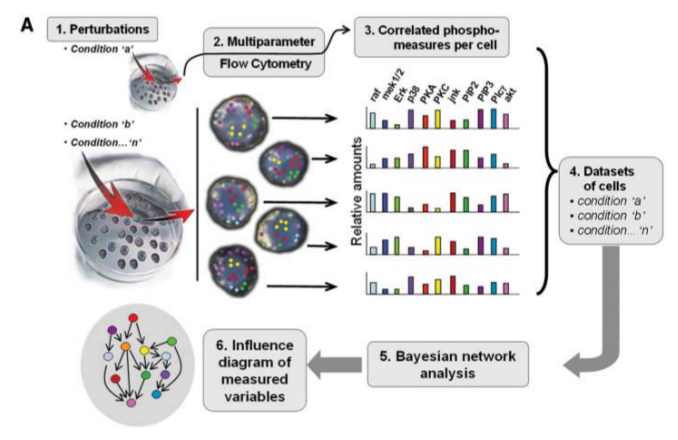
\includegraphics[scale=0.3]{../images/cytoA.png}
\end{center}
\begin{itemize}
\item Flow cytometry data from Sachs et al.\emph{Science}, 2005.
\item 1 observational data set + 9 interventions.
\end{itemize}
\end{frame}

\begin{frame}
\frametitle{Putative causal model}
\begin{center}
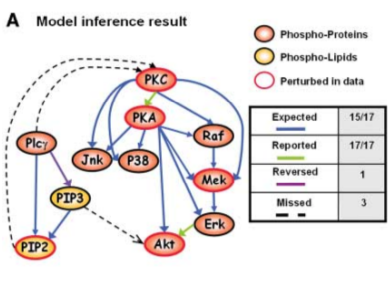
\includegraphics[scale=0.5]{../images/cyto_result_cropped.png}
\end{center}
\begin{itemize}
\item Causal inference applied to observational + interventional data.
\item Recovered most of the known interactions.
\end{itemize}
\end{frame}

\begin{frame}
\frametitle{The many facets of causality}
\begin{itemize}
\item \emph{Philosophy.} What is causality?  How do we learn about cause and effect? \emph{Aristotle, Hume.}
\item \emph{Computer science.}  Can we build an artificial intelligence which reasons like humans? \emph{Judea Peal.}
\item \emph{Social science.}  What influences an individual's life choices? 
\item \emph{Law.} Whose ``fault'' is it??
\item \emph{Statistics.} Answering the above questions using data!
\end{itemize}
\end{frame}

\begin{frame}
\frametitle{Statistics and causality}
\begin{itemize}
\item \emph{Estimating causal effects from data.} Can we predict a causal effect based on observational or experimental data? 
E.g. effect of a medical treatment based on clinical trial data?
Motviation for potential outcomes approach developed by Rubin, etc.
\item \emph{Bayesian networks/structure learning from data.} Can we model multivariate relationships using a network structure?
Networks \emph{can be} given causal interpretation, but causal inference is not the only motivation.
Motivation for graphical lasso.
\end{itemize}
\end{frame}

\begin{frame}
\sectionpage

\emph{Graphical approach} pioneered by Judea Pearl.

\begin{center}
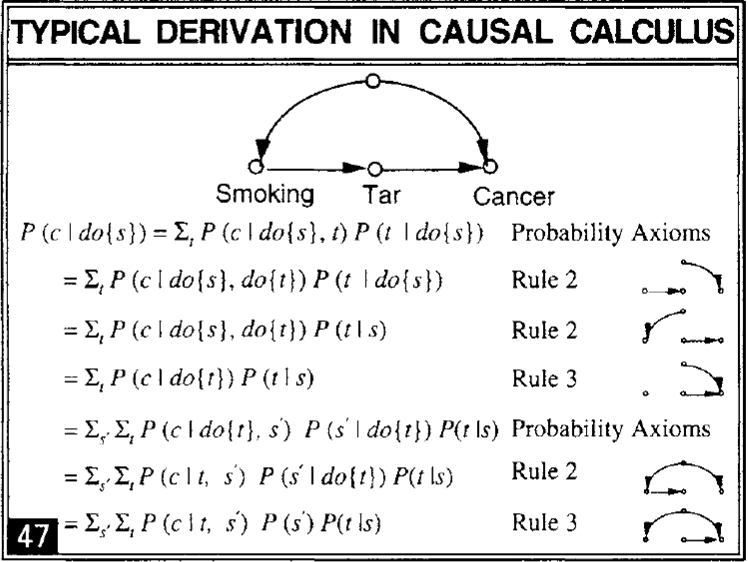
\includegraphics[scale = 0.2]{../images/pearl47.png}
\end{center}

\end{frame}

\begin{frame}
\frametitle{Graphs: nodes and vertices}

\begin{center}
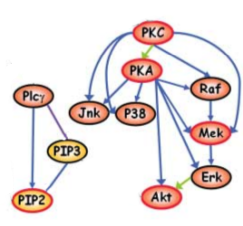
\includegraphics[scale = 0.5]{../images/cyto_result_cropped3.png}
\end{center}

\begin{itemize}
\item Each variable in the dataset is given a \emph{node}.
\item Arrows indicate which variables \emph{cause} which other variables. (Parents $\to$ children).
\item Undirected or bidirected edges = correlation due to mutual causation or latent common causes.
\end{itemize}

\end{frame}

\begin{frame}
\frametitle{Causality and experiments}
\begin{center}
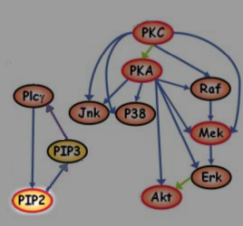
\includegraphics[scale = 0.5]{../images/fig01_01.png}
\end{center}

\emph{Intervening} on variables in the system causes the distribution to change.


\end{frame}

\begin{frame}
\frametitle{Causality and experiments}

\begin{center}
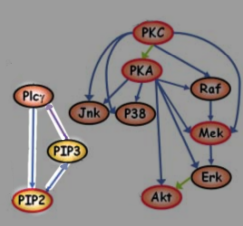
\includegraphics[scale = 0.5]{../images/fig01_02.png}
\end{center}

\begin{itemize}
\item Not every variable will be affected by the intervention!
\item Following the arrows tells you \emph{which} variables which are affected.
\end{itemize}

\end{frame}

\begin{frame}
\frametitle{Principle I: Which variables are affected.}

\begin{center}
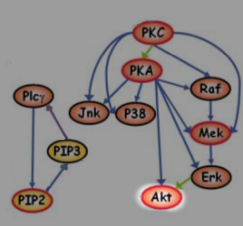
\includegraphics[scale = 0.5]{../images/fig01_03.png}
\hspace{0.5in}
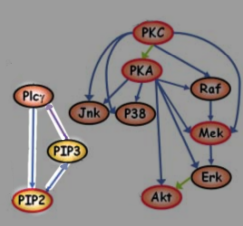
\includegraphics[scale = 0.5]{../images/fig01_02.png}
\end{center}

\begin{itemize}
\item If we \emph{inhibit} Akt, no other variables should be affected.
\item If we \emph{inhibit} PIP2, then we may not only change the distribution of PIP2, but also PIP3.
\end{itemize}

\end{frame}

\begin{frame}
\frametitle{Principle I: Which variables are affected.}

\begin{center}
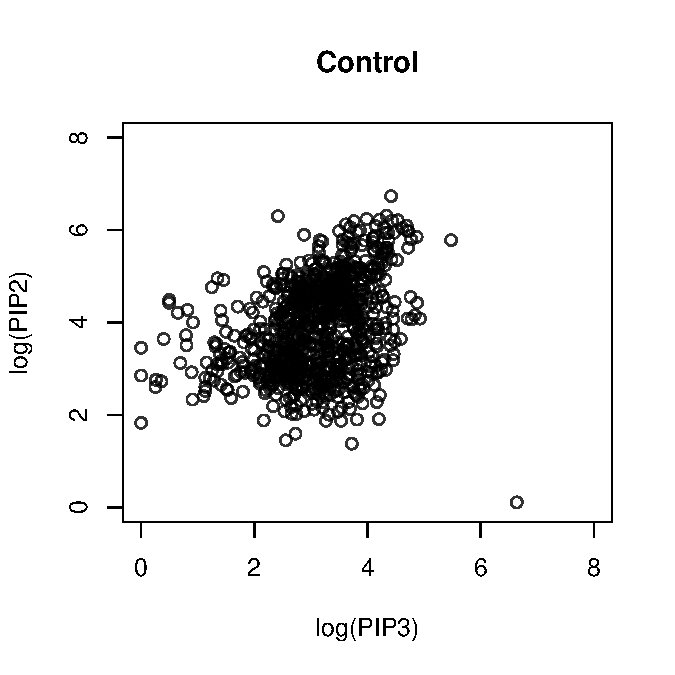
\includegraphics[scale = 0.5]{../images/plot01_01.pdf}
\end{center}

Looking at Sachs data.

Joint distribution of PIP2 and PIP3 in the ``control'' case.

\end{frame}


\begin{frame}
\frametitle{Principle I: Which variables are affected.}

\begin{center}
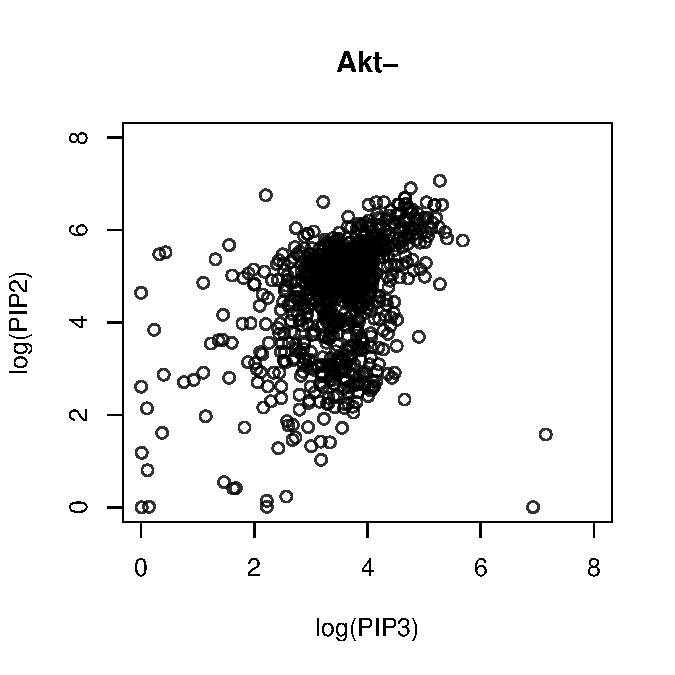
\includegraphics[scale = 0.5]{../images/plot01_02.pdf}
\end{center}

Joint distribution of PIP2 and PIP3 when we intervene on Akt.

\end{frame}

\begin{frame}
\frametitle{Principle I: Which variables are affected.}

\begin{center}
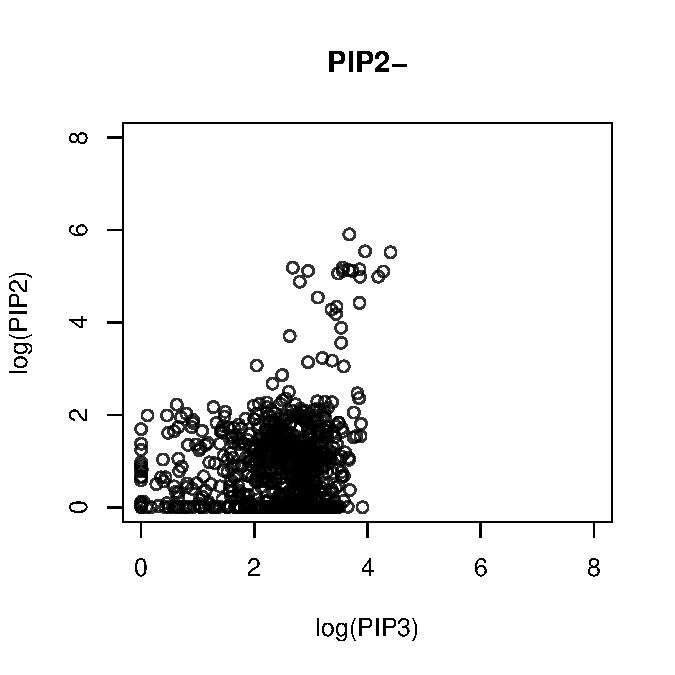
\includegraphics[scale = 0.5]{../images/plot01_03.pdf}
\end{center}

Joint distribution of PIP2 and PIP3 when we intervene on PIP2.

\end{frame}

\begin{frame}
\frametitle{Principle I: Which variables are affected.}

\begin{center}
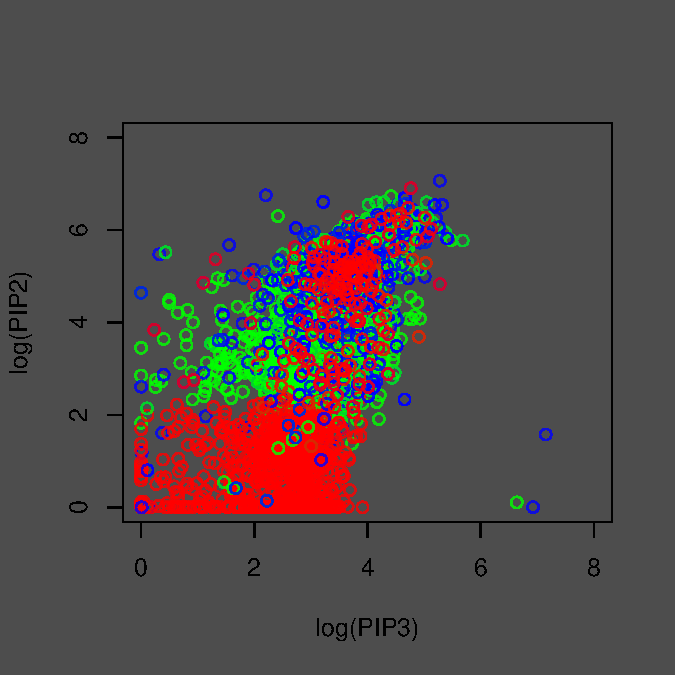
\includegraphics[scale = 0.5]{../images/plot01_04.pdf}
\end{center}

\begin{center}
\sethlcolor{color3}
\textbf{\textcolor{white}{\SoulColor\hl{ Control }}},
\sethlcolor{color1}
\textbf{\textcolor{white}{\SoulColor\hl{ PIP2- }}}, 
\sethlcolor{color2}
\textbf{\textcolor{white}{\SoulColor\hl{ Akt- }}}
\end{center}

Intervening on PIP2 also affects the distribution of PIP3,
while intervening on Akt does not (drastically) change the distribution.

\end{frame}


\begin{frame}
\frametitle{Principle II: Conditional independence.}

\begin{center}
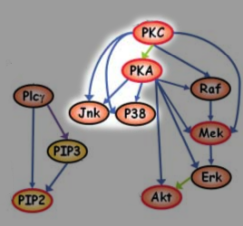
\includegraphics[scale = 0.5]{../images/fig03_01.png}
\end{center}

\begin{itemize}
\item Surprisingly, the structure of the causal graph implies certain \emph{conditional independence} relationships.
\item This allows the potential to infer causal relationships from observational data.
\end{itemize}

\end{frame}

\begin{frame}
\frametitle{Principle II: Conditional independence.}

\begin{center}
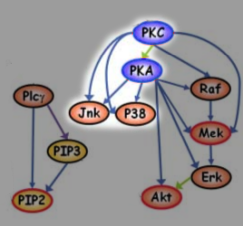
\includegraphics[scale = 0.5]{../images/fig03_02.png}
\end{center}

\begin{itemize}
\item Two variables are independent conditional on their common parents.
\item Conditioning on PKC and PKA, Jnk and p38 should be independent.
\end{itemize}

\end{frame}


\begin{frame}
\frametitle{Principle II: Conditional independence.}

\begin{center}
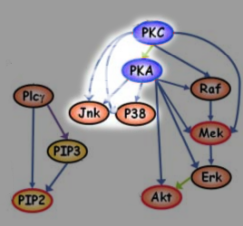
\includegraphics[scale = 0.5]{../images/fig03_03.png}
\end{center}

\begin{itemize}
\item ``Once you and I condition on common factors, we are left with nothing in common.''
\end{itemize}

\end{frame}

\begin{frame}
\frametitle{Principle II: Conditional independence.}

\begin{center}
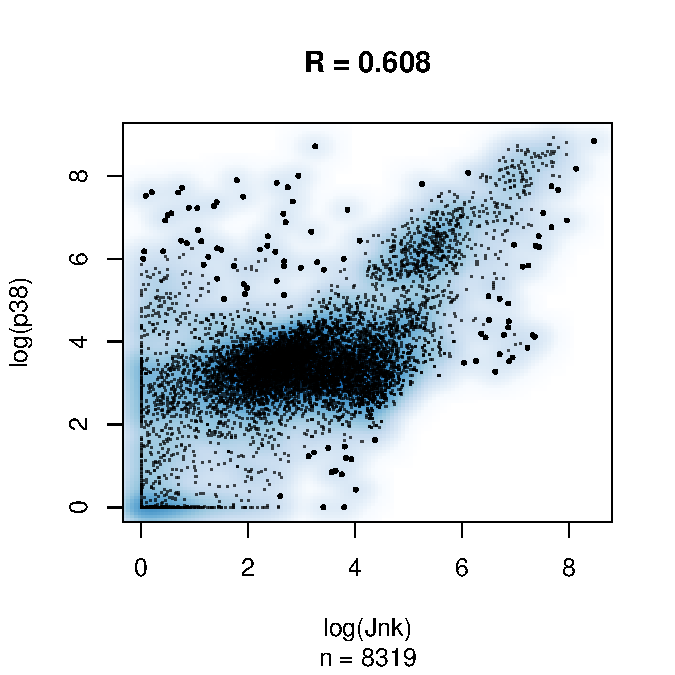
\includegraphics[scale = 0.5]{../images/plot03_01.pdf}
\end{center}

Marginally, p38 and Jnk are correlated.

\end{frame}

\begin{frame}
\frametitle{Principle II: Conditional independence.}

\begin{center}
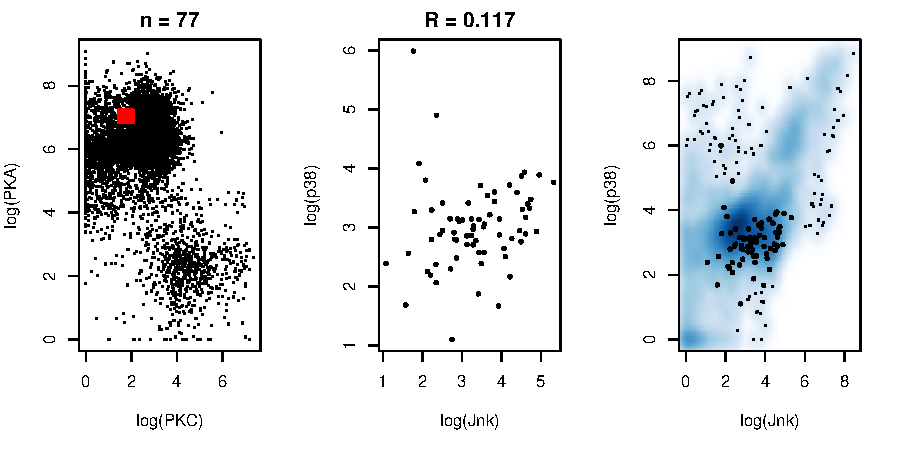
\includegraphics[scale = 0.7]{../images/plot03_02.pdf}
\end{center}

We can't condition on PKA and PKC since the data is continuous.
But, conditioning on small windows seems to reduce association.

\end{frame}


\begin{frame}
\frametitle{Principle II: Conditional independence.}

\begin{center}
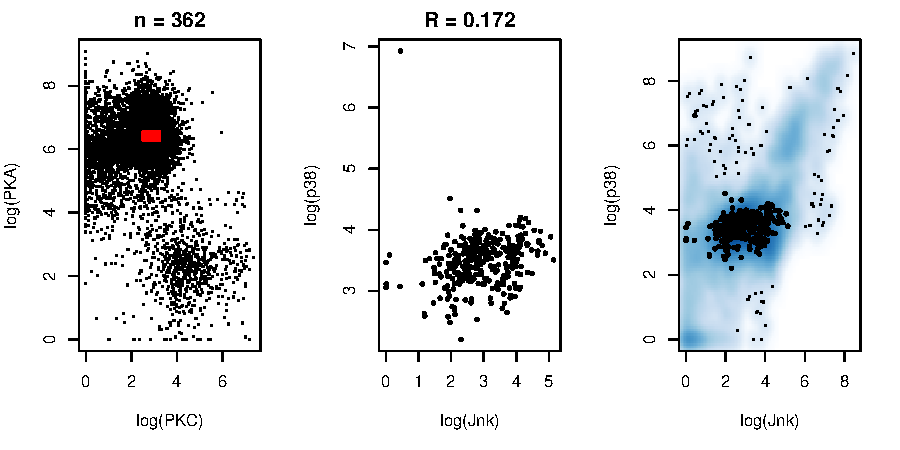
\includegraphics[scale = 0.7]{../images/plot03_03.pdf}
\end{center}

\emph{Left:} We condition on (PKA, PKC) to lie within the indicated window.
\emph{Center:} Conditional joint distribution of (Jnk, p38).
\emph{Right:} Conditional join distribution, overlaid on marginal distribution.
\end{frame}

\begin{frame}
\frametitle{Principle II: Conditional independence.}

\begin{center}
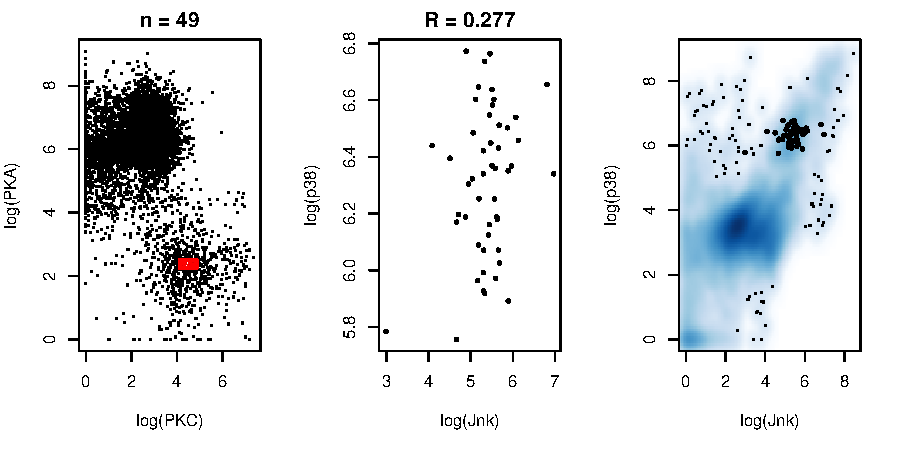
\includegraphics[scale = 0.7]{../images/plot03_04.pdf}
\end{center}

PKA and PKC \emph{explain away} some (if not all) of the association between Jnk and p38.
(Recall that R = 0.608 marginally.)

\end{frame}


\begin{frame}
\frametitle{Principle III: Predictive invariance}

\begin{center}
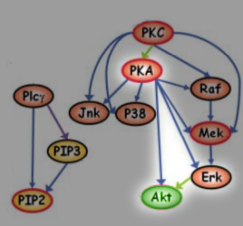
\includegraphics[scale = 0.5]{../images/fig04_01.png}
\end{center}

%A principle brought to attention by a recent paper by the ``Zurich group'' (Peters Meinshausen, Buhlmann).

\begin{itemize}
\item The conditional distribution $\Pr[Akt|PKA, Erk]$ is invariant to interventions applied to other variables.
\item Therefore, the optimal rule for predicting $\hat{Akt}(PKA, Erk)$ is invariant as well.
\end{itemize}
\end{frame}

\begin{frame}
\frametitle{Principle III: Predictive invariance}
\begin{center}
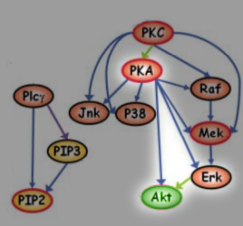
\includegraphics[scale = 0.5]{../images/fig04_01.png}
\end{center}

$\{PKA, Erk\}$ is an ``invariant set'' for $Akt$ since:

\begin{itemize}
\item It includes all of the ``direct'' causes of $Akt$ in the graph.
\item It doesn't include any variables caused by $Akt$.
\end{itemize}

\end{frame}

\begin{frame}
\frametitle{Principle III: Predictive invariance}
\begin{center}
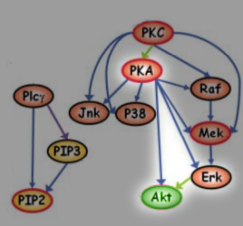
\includegraphics[scale = 0.5]{../images/fig04_01.png}\hspace{0.5in}
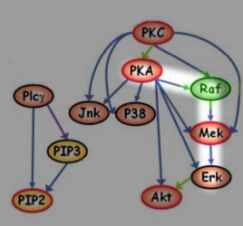
\includegraphics[scale = 0.5]{../images/fig05_01.png}
\end{center}

In contrast, $\{PKA, Mek, Erf\}$ is \emph{not} an invariant set for $Raf$ since:

\begin{itemize}
\item .
\item .
\end{itemize}

\end{frame}






\begin{frame}
\frametitle{Principle III: Predictive invariance}
\begin{center}
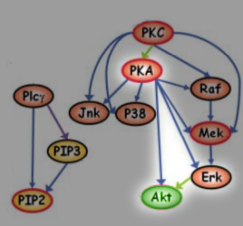
\includegraphics[scale = 0.5]{../images/fig04_01.png}\hspace{0.5in}
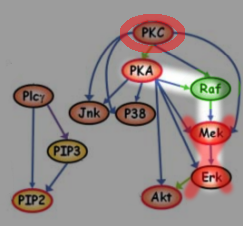
\includegraphics[scale = 0.5]{../images/fig05_02.png}
\end{center}

In contrast, $\{PKA, Mek, Erf\}$ is \emph{not} an invariant set for $Raf$ since:

\begin{itemize}
\item It is missing a direct cause of $Raf$.
\item It contains variables which are caused by $Raf$.
\end{itemize}

\end{frame}





\begin{frame}
\frametitle{$\{PKA, Erk\}$ is an invariant set for $Akt$.}
\begin{center}
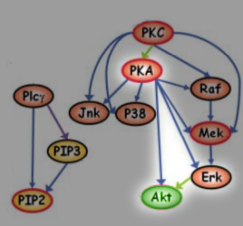
\includegraphics[scale = 0.3]{../images/fig04_01.png}\hspace{0.5in}
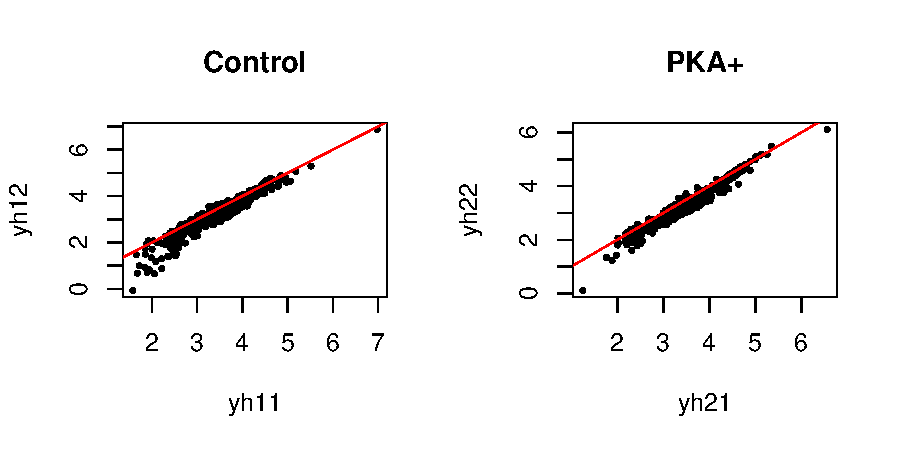
\includegraphics[scale = 0.6]{../images/plot04_01.pdf}
\end{center}
\end{frame}





\begin{frame}
\frametitle{$\{PKA, Mek, Erf\}$ is \emph{not} an invariant set for $Raf$.}
\begin{center}
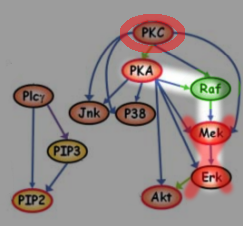
\includegraphics[scale = 0.3]{../images/fig05_02.png}\hspace{0.5in}
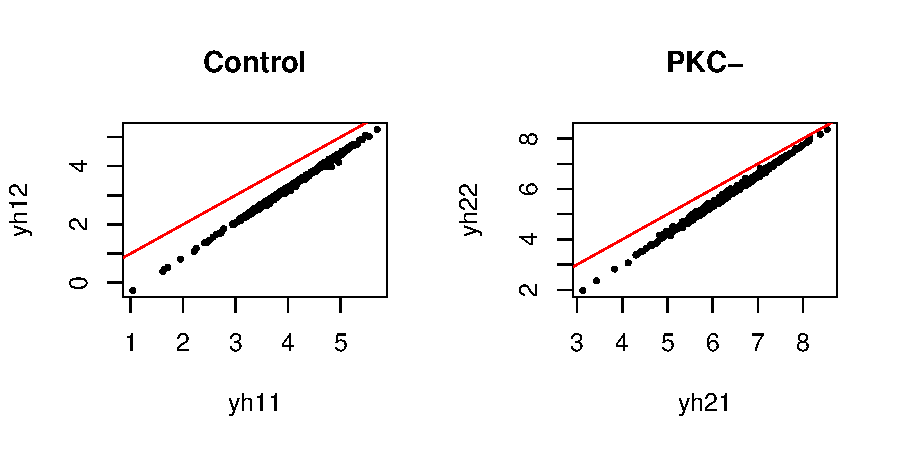
\includegraphics[scale = 0.6]{../images/plot05_01.pdf}
\end{center}
\end{frame}



\begin{frame}
\frametitle{Predictive Invariance: Example}
\begin{center}
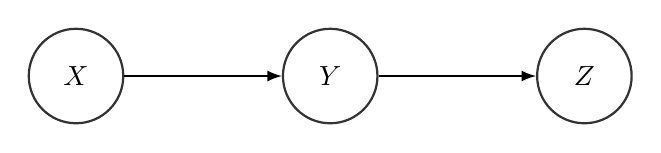
\begin{tikzpicture}[node distance = 2mm and 20mm]
\tikzstyle{main} = [circle, minimum size = 12mm, thick, draw = black!80]
\tikzstyle{connect} = [-latex, thick]
  \node[main] (x) {$X$};
  \node[main, right=of x] (y) {$Y$};
  \node[main, right=of y] (z) {$Z$};
\path (x) edge [connect] (y) (y) edge [connect] (z);
\end{tikzpicture}
\end{center}
\begin{itemize}
\item Suppose we are trying to predict $Y$.
\item $X \sim N(0, a)$.
\item $Y|X \sim N(X, b)$.
\item $Z|Y \sim N(Y, c).$
\end{itemize}
\end{frame}


\begin{frame}
\frametitle{Predictive Invariance: Example}
\begin{center}
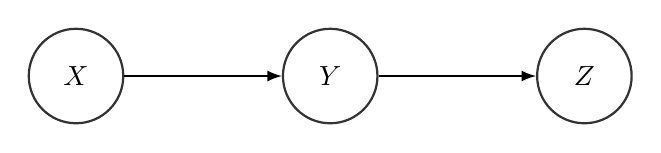
\begin{tikzpicture}[node distance = 2mm and 20mm]
\tikzstyle{main} = [circle, minimum size = 12mm, thick, draw = black!80]
\tikzstyle{connect} = [-latex, thick]
  \node[main] (x) {$X$};
  \node[main, right=of x] (y) {$Y$};
  \node[main, right=of y] (z) {$Z$};
\path (x) edge [connect] (y) (y) edge [connect] (z);
\end{tikzpicture}
\[X \sim N(0, a),\ Y|X \sim N(X, b),\ Z|Y \sim N(Y, c).\]
\end{center}
\begin{itemize}
\item We can intervene by adding noise to $X$ = changing $a \to a'$.
\item Intervene by injecting noise to $Z$ = changing $c \to c'$.
\item Consider a linear model which predicts $Y$ given $X$ and $Z$.
\item \emph{Is the optimal prediction rule invariant under intervention?}
\end{itemize}
\end{frame}


\begin{frame}
\frametitle{Predictive Invariance: Example}
\begin{center}
\[X \to Y \to Z\]
\[X \sim N(0, a),\ Y|X \sim N(X, b),\ Z|Y \sim N(Y, c).\]
\end{center}

The joint distribution is 
\[
\begin{bmatrix}
X \\ Y\\Z
\end{bmatrix}
\sim
N\left(
\begin{bmatrix}
0 \\ 0 \\ 0
\end{bmatrix},
\begin{bmatrix}
a & a & a \\
a & a + b & a + b\\
a & a + b & a + b + c
\end{bmatrix}
\right)
\]

The optimal prediction rule is given by
\[
\E[Y|X, Z] = \mu_Y + \Sigma_{Y, XZ}\Sigma_{XZ}^{-1} (X - \mu_X, Z - \mu_Z) = \frac{c}{b + c} X + \frac{b}{b+c} Z.
\]

\end{frame}


\begin{frame}
\frametitle{Predictive Invariance: Example}
\begin{center}
\[X \sim N(0, a),\ Y|X \sim N(X, b),\ Z|Y \sim N(Y, c).\]
\end{center}

Optimal prediction rule:
\[
\E[Y|X, Z] = \underbrace{\frac{c}{b+c}}_{\beta_X} X + \underbrace{\frac{b}{b+c}}_{\beta_Z} Z.
\]

i.e. $Y$ is a weighted average of $X$ and $Z$ ($\beta_X + \beta_Z = 1$).

\begin{itemize}
\item Imagine $c$ is very small, i.e. $Z$ = $Y$ + tiny noise.  Then $Z$ is a great predictor of $Y$!  $\beta_Z \approx 1$.
\item Conversely, if $b$ is small, that means $Y$ = $X$ + tiny noise.  $\beta_X \approx 1$.
\item If $b = c$, then $\beta_X = \beta_Z = 1/2$.
\end{itemize}

\end{frame}






\begin{frame}
\frametitle{Predictive Invariance: Example}

But is the OLS predictive rule invariant?
\[
\E[Y|X, Z] = \frac{c}{b + c} X + \frac{b}{b+c} Z.
\]
If we intervene on $Z$, changing $c$ to $c'$, the OLS coefficients change too.
The model is not invariant.

\begin{center}
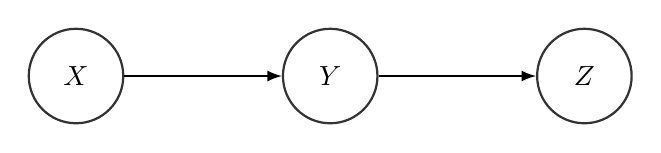
\begin{tikzpicture}[node distance = 2mm and 20mm]
\tikzstyle{main} = [circle, minimum size = 12mm, thick, draw = black!80]
\tikzstyle{connect} = [-latex, thick]
  \node[main] (x) {$X$};
  \node[main, right=of x] (y) {$Y$};
  \node[main, right=of y] (z) {$Z$};
\path (x) edge [connect] (y) (y) edge [connect] (z);
\end{tikzpicture}
\end{center}

\emph{``Real-life'' example.}
$X = $ how much you weigh? $Y = $ how many bagels you eat every day? $Z= $ how many pull-ups you can do?

$Z$ is a good predictor of $Y$, unless you ``intervene'' by offering a \$100 prize for doing 10 pull-ups.

\end{frame}

\begin{frame}
\frametitle{Predictive Invariance: Example}
\begin{center}
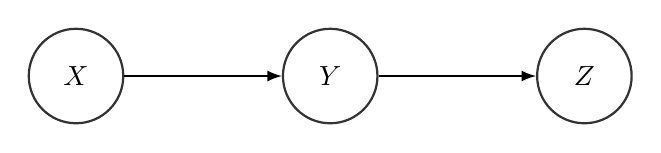
\begin{tikzpicture}[node distance = 2mm and 20mm]
\tikzstyle{main} = [circle, minimum size = 12mm, thick, draw = black!80]
\tikzstyle{connect} = [-latex, thick]
  \node[main] (x) {$X$};
  \node[main, right=of x] (y) {$Y$};
  \node[main, right=of y] (z) {$Z$};
\path (x) edge [connect] (y) (y) edge [connect] (z);
\end{tikzpicture}
\end{center}
\begin{itemize}
\item In contrast, consider predicting $Y$ using \emph{only} $X$.
\item $\{X\}$ is an invariant set for $Y$ because it contains all direct parents and no children of $Y$.
\item Indeed,
\[
\E[Y|X] = \frac{\Cov(Y, X)}{\Cov(X)} X = \frac{a}{a} X = X.
\]
The OLS coefficient, 1, does not depend on $a$ or $c$, and hence is \emph{invariant} under interventions.
\item \emph{Exercise.} Is $\{Z\}$ an invariant set for $Y$?
\end{itemize}
\end{frame}




\begin{frame}
\frametitle{Overview: Principles of Causal Inference}
Causal relationships in a system represented by a graph.  The graph tells you:
\begin{itemize}
\item[I.] which variables are affected by an intervention.
\item[II.] what conditional independence relationships exist in the joint distribution.
\item[III.] which sets of predictors and responses will have ``invariant'' optimal predictive rules.
\end{itemize}
\end{frame}

\section{Statistical Methods}

\begin{frame}
\sectionpage
\end{frame}


\begin{frame}
\frametitle{Estimating Causal Effects}
\begin{center}
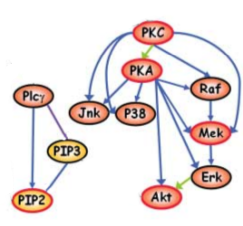
\includegraphics[scale = 0.5]{../images/cyto_result_cropped3.png}
\end{center}

\begin{itemize}
\item Suppose we want to reduce the expression level of PKC in the cell.  We have a treatment (an enzyme) which can inhibit PIP2-- what would be the \emph{treatment effect}
\[
\E[PKC | do(PIP2)] - \E[PKC] = ?
\]
\end{itemize}
\end{frame}



\begin{frame}
\begin{itemize}
\item \emph{Controlled experiment.} Do an experiment where we randomize the treatment, estimate the treatment effect using the difference
\[
\text{mean of the treated} - \text{mean of the controls}
\]
\item \emph{Observational data.}  We observe that the enzyme we are considering is sometimes expressed in the cell naturally.  Can we estimate the treatment effect even without having done a controlled experiment?
\begin{itemize}
\item \emph{Potential outcomes approach.} (By Rubin et al.)  Match treated and untreated observations using \emph{propensity scores.}  Optional: sensitivity analyses.
\item \emph{Graphical approach.}  (Pearl et al.)  Supposing we know the structure of the graph (or we can try to learn it), apply \emph{calculus of interventions.}
\end{itemize}
\end{itemize}
\end{frame}


\begin{frame}
\frametitle{Observational data}
\begin{center}
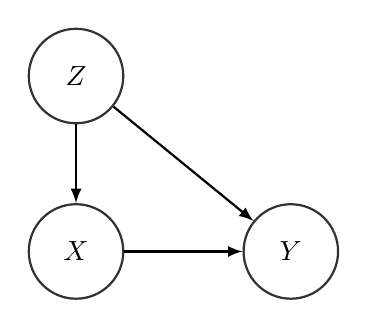
\begin{tikzpicture}[node distance = 10mm and 15mm]
\tikzstyle{main} = [circle, minimum size = 12mm, thick, draw = black!80]
\tikzstyle{connect} = [-latex, thick]
  \node[main] (x) {$X$};
  \node[main, right=of x] (y) {$Y$};
  \node[main, above=of x] (z) {$Z$};
\path (x) edge [connect] (y) (z) edge [connect] (y) (z) edge [connect] (x);
\end{tikzpicture}
\end{center}
\begin{itemize}
\item $X = \{0, 1\}$ is the treatment variable, $Y$ is the outcome of interest, $Z$ are confounders.
\item Want to estimate effect of treatment.
\item No confounders?? Use $\E[Y|X=1] - \E[Y|X = 0]$, done!
\item \emph{Unobserved} confounders?!  We'll discuss next time..
\item For now, assume all confounders are observed.
\end{itemize}
\end{frame}

\begin{frame}
\frametitle{Calculus of interventions}
\begin{itemize}
\item Our goal is to infer the average treatment effect,
\[
\E[Y|do(X=1)] - \E[Y|do(X = 0)]
\]
\item The `do' notation refers to interventions.
\item We have observational data,
\[p(x, y, z) = p(y|x,z)p(x|z)p(z).\]
\end{itemize}
\begin{center}
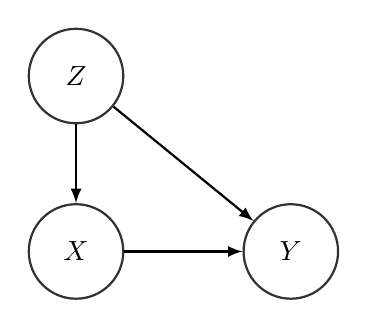
\begin{tikzpicture}[node distance = 10mm and 15mm]
\tikzstyle{main} = [circle, minimum size = 12mm, thick, draw = black!80]
\tikzstyle{connect} = [-latex, thick]
  \node[main] (x) {$X$};
  \node[main, right=of x] (y) {$Y$};
  \node[main, above=of x] (z) {$Z$};
\path (x) edge [connect] (y) (z) edge [connect] (y) (z) edge [connect] (x);
\end{tikzpicture}
\end{center}

\end{frame}

\begin{frame}
\frametitle{Adjustment for confounders}
To compute $\E[y|do(X=1)] - \E[y|do(X=0)]$, it suffices to estimate $p(y|do(x))$.
\begin{itemize}
\item $p(x, y, z) = p(y|x,z)p(x|z)p(z).$
\item Step one: convert between `do' notation and probability
\[
p(y | x, z) = p(y | do(x), z).
\]
\item Step two: apply law of total probability
\[
p(y|do(x)) = \sum_z p(y, z|do(x)) = \sum_z p(y|do(x), z) p(z|do(x))\]\[ = \sum_z p(y|x, z) p(z).
\]
\item Step three: plug in empirical $\hat{p}(y|x, z)$ obtained by conditioning on $z$.
\end{itemize}
\end{frame}

\begin{frame}
\frametitle{Potential outcomes formulation}
Potential outcomes uses notation $Y^{(0)}$ for $Y|do(X=0)$ and $Y^{(1)}$ for $Y|do(X = 1)$.
\begin{itemize}
\item First, determine the nature of the ``assignment mechanism,'' $X$.  In this case, the probability that $X=1$ is determined by $Z$,
$f(z) = p(X=1|z).$
The function $f(z)$ is called the \emph{propensity score.}
\item Estimate $f(z)$ using regression (e.g. logistic regression $X$ on $Z$).
\item Match `cases'  (which have $X=1$) to `controls' (with $X=0$) that have similar propensity scores.
\item Compute average treatment effect by a weighted average of:
\[
\Pr[X=1]\underbrace{(\E[Y|X=1] - \E[Y|do(X=0), X=1])}_{\text{treatment effect on treated}}\]\[
+\Pr[X=0]\underbrace{(\E[Y|X=0, do(X=1)] - \E[Y|X=0])}_{\text{treatment effect on untreated}}
\]
\end{itemize}
\end{frame}

\begin{frame}
\frametitle{Comparison of approaches}
\begin{itemize}
\item Approaches are \emph{almost} equivalent in this example.
Matching based on $f(z)=p(x|z)$ and weighting based on probability of treatment
produces the same result as conditioning on $Z$.
\item Practically, there are still subtle differences.  Easier to get confidence intervals in one approach than another, etc.
\item The real devil is in the assumptions of the approaches.  Which assumptions are needed, and how can they be checked?
How much knowledge about the graph do we need for each approach?
\end{itemize}
\end{frame}

\begin{frame}
\section{Conclusions}
\sectionpage
\begin{itemize}
\item Causal models imply statements about which variables get affected by interventions,
which conditional independencies exist, and which sets of variables lead to invariant prediction rules.
\item Real data may reveal a causal model to be more of a useful approximation than a literal description.
\item Estimation of causal effects from experiments with imperfect randomization or observational data is a common goal in causal inference, and can be addressed using the graphical approach or potential outcomes framework.
\end{itemize}
\end{frame}


\begin{frame}
\frametitle{Next time...}
In part II of the talk, we'll go into more detail about the limitations of causal inference, and criticism of many common practices.
\begin{itemize}
\item Does causal inference require us to make too many strong assumptions?
\item Do instrumental variable approaches give sensible results?
\item How robust are causal inferences to hidden confounders?
\item Is it realistic to be able to learn structure from completely observational data?
\end{itemize}

We'll also introduce the causal invariance approach by Peters, Meinshausen, and B\"{u}hlmann--could this new approach extend the applicability of causal inference?

\end{frame}

\begin{frame}
\frametitle{Reference}
\begin{itemize}
\item Peters, Jonas, Peter B\"{u}hlmann, and Nicolai Meinshausen. ``Causal inference using invariant prediction: identification and confidence intervals.'' arXiv preprint arXiv:1501.01332 (2015).
\end{itemize}
\end{frame}



\end{document}






